\chapter{ECG Arrhythmias classification} \label{chap5}

\section{Centralized Learning} \label{5CL}

To get an understanding of the best performances achievable with the mentioned dataset I implemented Centralized (or traditional) Learning. The latter means that I applied the analytical tools mentioned in \ref{chap4} over the complete dataset, without dividing it into clients. Then the main processes and results are summarized in the following phases.

\subsection{Data wrangling}

As mentioned in \ref{4dw}, the data wrangling process is usually the first step when dealing with a data-oriented problem. In this case, I placed the data in a Google Drive folder after downloading it from the official competition's website \cite{dataset3}. Afterwards, using Google Colaboratory I extracted and organized the information in Python. The representation of the ECG along the 12-leads can be examined in Figure \ref{fig:ecg_example_S0033}.

\begin{figure}[H]
\centering
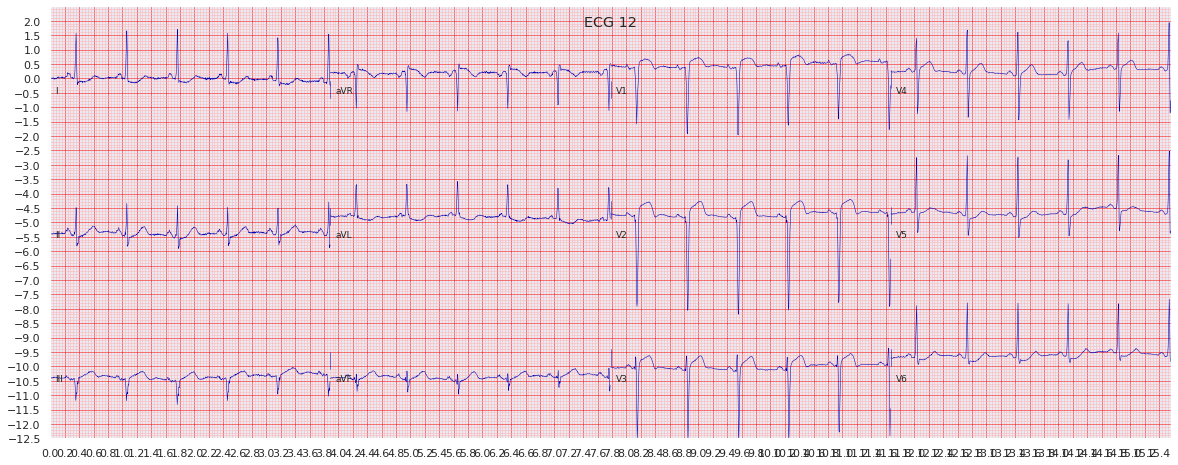
\includegraphics[scale=0.32]{img/ecg_example_S0033.png}
\caption{12-lead ECG for recording S0033 of PTB database}
\label{fig:ecg_example_S0033}
\end{figure}

Then, the whole data (all the databases) and the features mentioned in \ref{4fe} was calculated. That process took almost 1 hour to run and used the default configuration of Google Colab. Besides, for each recording, I selected the first diagnosis (arrhythmia) that appeared as the label to be predicted. The latter process ran in about 2 minutes.

\subsection{EDA}

Once the big dataset was loaded, it contained a total of 43,101 recordings and about 764 variables. From the latter, 650 features got created containing 14 competition-provided features and 636 were spectral features. There were remaining 3 corresponded to the id of the recording, the database that it belongs to and the label (response variable to be predicted). Then, the first analysis needed was to examine if the features contained any missing values. Using the function \texttt{bar} from the \texttt{missingno} library, I managed to explore the missing values. In figure \ref{fig:eda_missing} are depicted only the 50 first features' missing counts and percentages.

\begin{figure}[H]
\centering
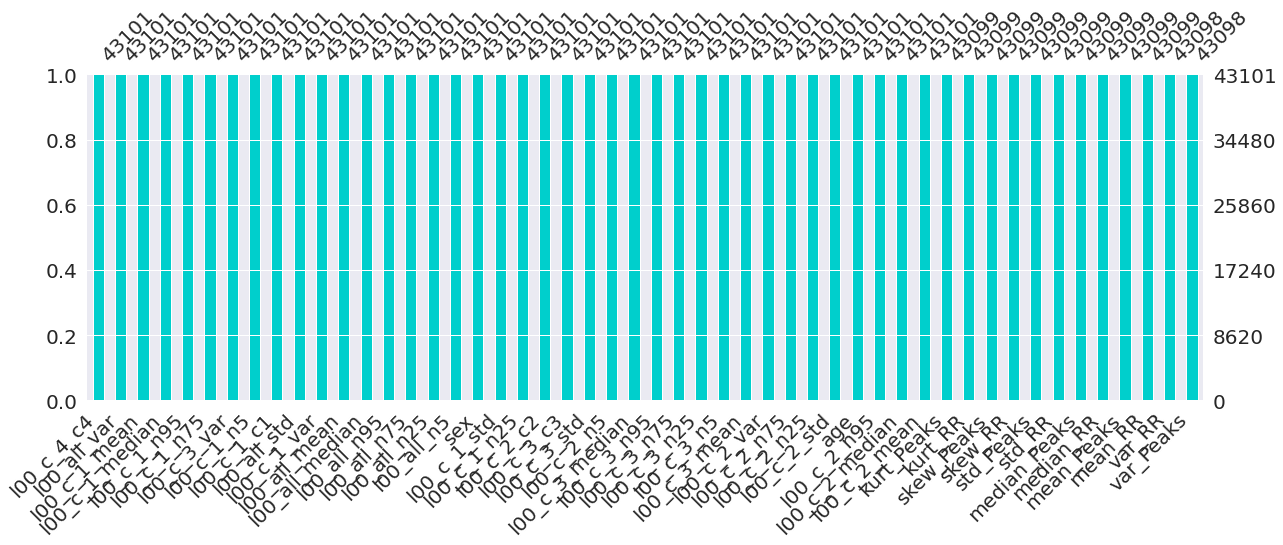
\includegraphics[scale=0.30]{img/eda_missing.png}
\caption{Missing counts and percentage for 50 features of the complete dataset}
\label{fig:eda_missing}
\end{figure}

As shown in the previous chart, the missing percentage is considerably small (less than 0.1\%). For that reason, I decided to impute those missing values by using the mean (average) of each attribute. 

The second crucial aspect to investigate was the distribution of the response variable. Then, within the plot \ref{fig:label_ditro_alldata} it is shown the absolute count of each diagnosis in the dataset.

\begin{figure}[H]
\centering
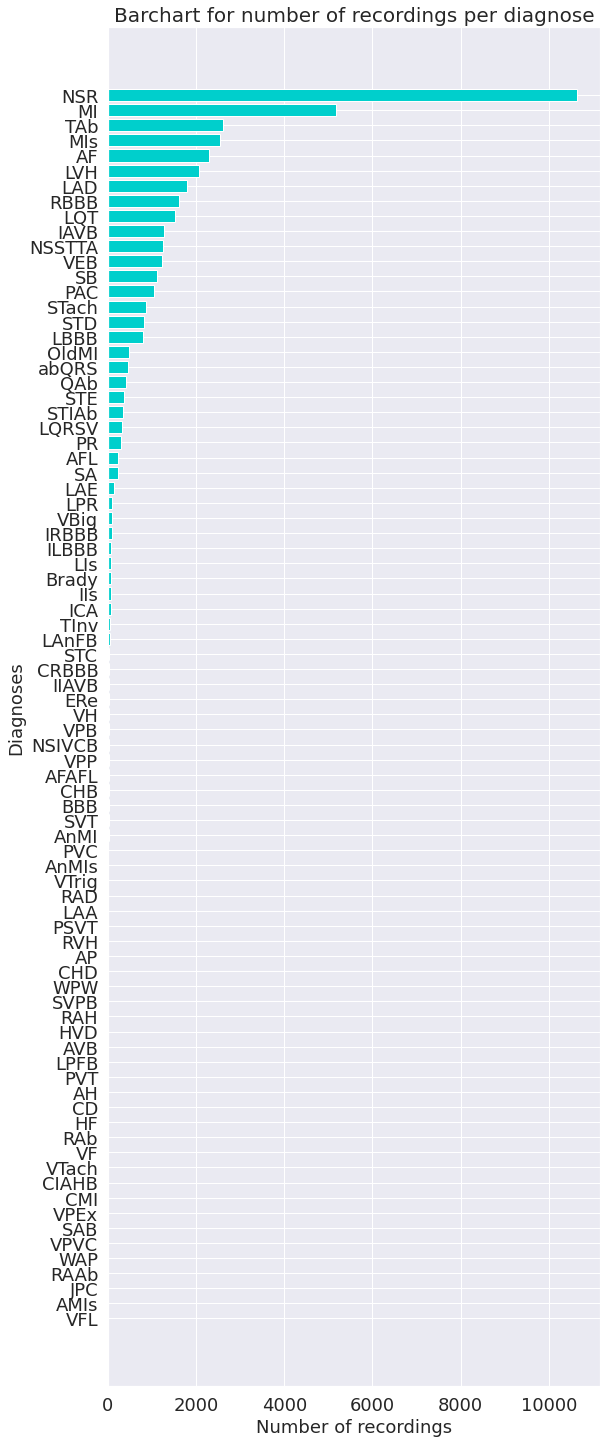
\includegraphics[scale=0.32]{img/label_ditro_alldata.png}
\caption{Label distribution for the complete dataset}
\label{fig:label_ditro_alldata}
\end{figure}

As evidenced in the previous chart, there are too many arrhythmias that don't have big participation. That can lead to problems when trying to infer the predicted class of a recording since there were not enough cases to learn the classifiers properly. That is why those diagnoses with participation smaller than 150 records were discarded from the analysis. With the previous filter, the selected data to work with got a size of 41,894 recordings distributed as shown in figure \ref{fig:diagnose_count_by_db_filtered}.

\begin{figure}[H]
\centering
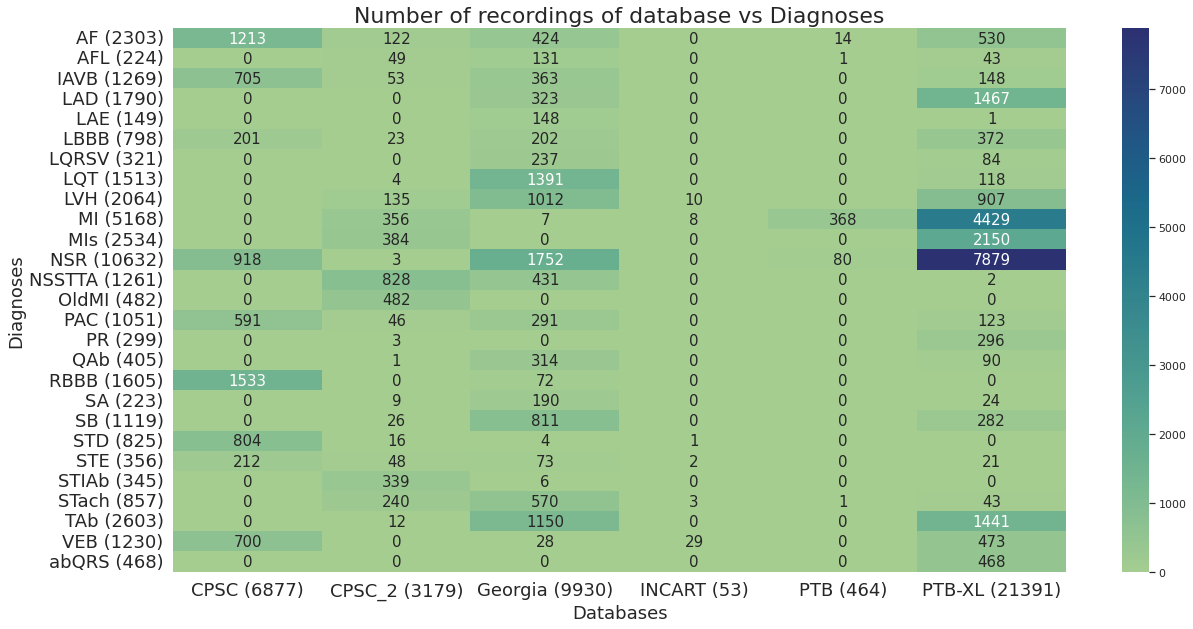
\includegraphics[scale=0.32]{img/diagnose_count_by_db_filtered.png}
\caption{Number of recordings for each diagnosis by database for the filtered data}
\label{fig:diagnose_count_by_db_filtered}
\end{figure}

Besides, the final distribution of the labels ended up as shown in figure \ref{fig:label_ditro_filtered}. As expected, the most common diagnosis was Normal Sinus Rhythm (NSR), which is the normal status for an ECG. In addition. the arrhythmia with one of the smallest participation turned out to be Sinus Arrhythmia (SA).

\begin{figure}[H]
\centering
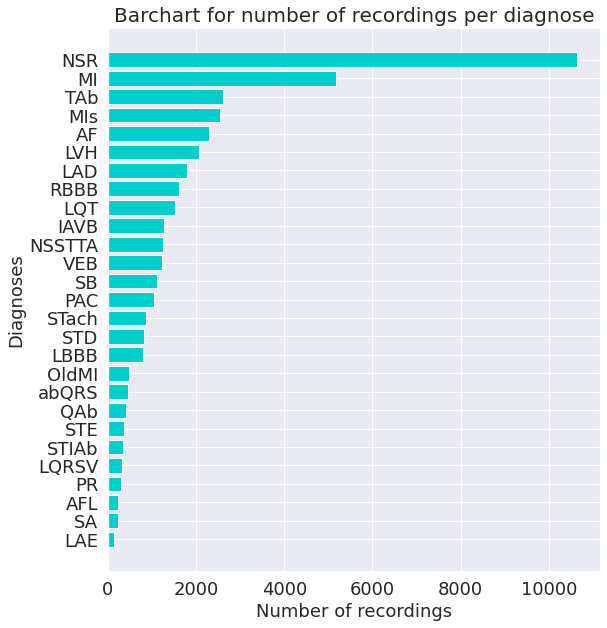
\includegraphics[scale=0.32]{img/label_ditro_filtered.png}
\caption{Label distribution for the filtered dataset}
\label{fig:label_ditro_filtered}
\end{figure}

\subsection{Feature Selection and normalization}\label{5fsn}

In an analytical context, having a huge amount is a double-edged sword. On the one hand, the more information exists to predict phenomena, the better. On the other hand, the computational time required to process too much information may lead to training times that are not affordable. Regarding the latter, I decided to perform a feature selection step to determine the most important features to predict arrhythmias. 

\begin{figure}[H]
\centering
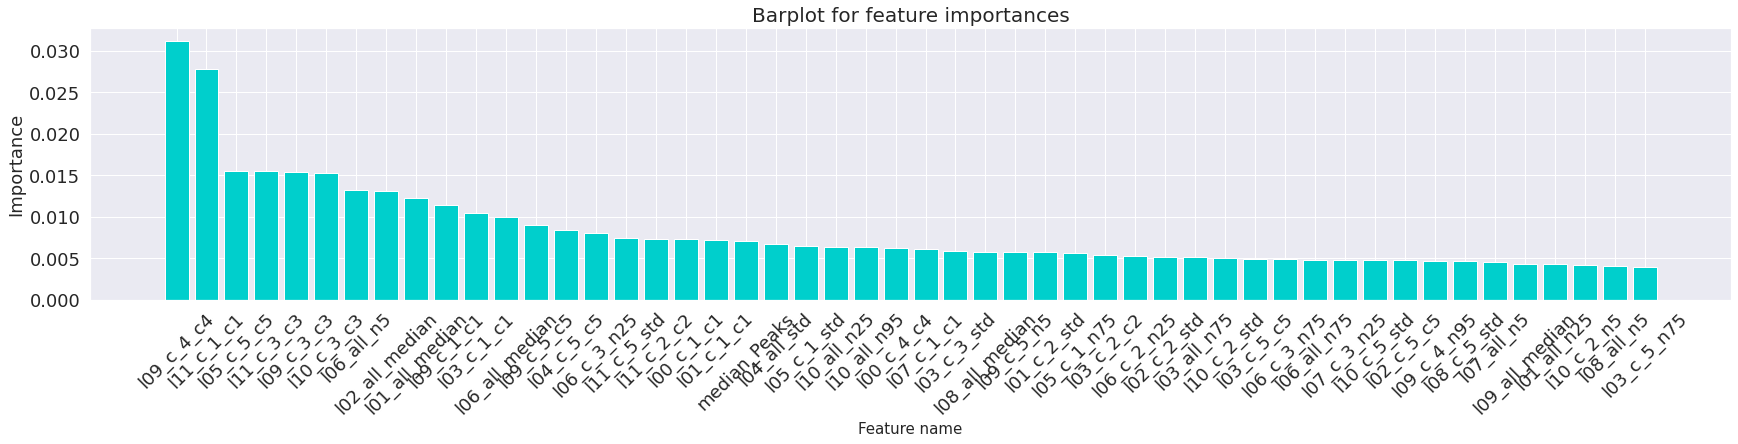
\includegraphics[scale=0.22]{img/feature_importance.png}
\caption{Feature importance from XG-Boost algorithm (only the 50 best)}
\label{fig:feature_importance}
\end{figure}

The bar-plot in figure \ref{fig:feature_importance} depicted the most important features to predict the classes obtained employing the XG-Boost method. The latter provides an automatic ranking of the most relevant features to classifier the ECGs. After having the importance of features of all 650 features, the next step was to try to reduce the unimportant features and
run the model. During the various trial run and keeping the F1-Score as the primary metric reducing ranked features from 150 -100 F1-score went down from 0.56 to 0.52 and keeping it on 120 features it goes back to 0.56. So, in the end, 120 features got selected which leads to good enough accuracy and f1-
score compared to the one obtained using all the features. The best features turned out to be the Entropy for leads: 9, 11, 10; the percentile 5\% for lead 6; and the median for leads 1, 2.

As an additional tool to enhance the performance of the models, there was an implementation of features \textbf{normalization}. In this case, I tried three different techniques to transform the features to the same scale. The approaches tried were provided by the \texttt{sklearn} library in Python. Those are: \texttt{StandardScaler}, \texttt{MaxMinScaler} and \texttt{RobustScaler}. In the end, the scenario that provided the best results was using \texttt{RobustScaler}. 

\begin{equation} \label{robustscaler_eq}
X_{scale} = \frac{x_i - x_{med}}{x_{75} - x_{25}}
\end{equation}

\texttt{RobustScaler} [\ref{robustscaler_eq}] uses statistics that was resistant to outliers to scale features. The median was removed, and the data were scaled according to the quantile range (defaults to IQR: Interquartile Range). The interquartile range (IQR) is the distance between the first and third quartiles (25th and 3rd quantiles) (75th quantile). It is worth mentioning that centering and scaling happen independently on each feature by computing the relevant statistics on the samples in the given dataset.

\subsection{Balancing classes (arrhythmias)}

As depicted in \ref{fig:label_ditro_filtered}, the diagnoses have a imbalanced characteristic. The latter means that each category has different participation in the data. That could represent a problem in the performance of the classifiers that will be proposed.

\begin{figure}[H]
\centering
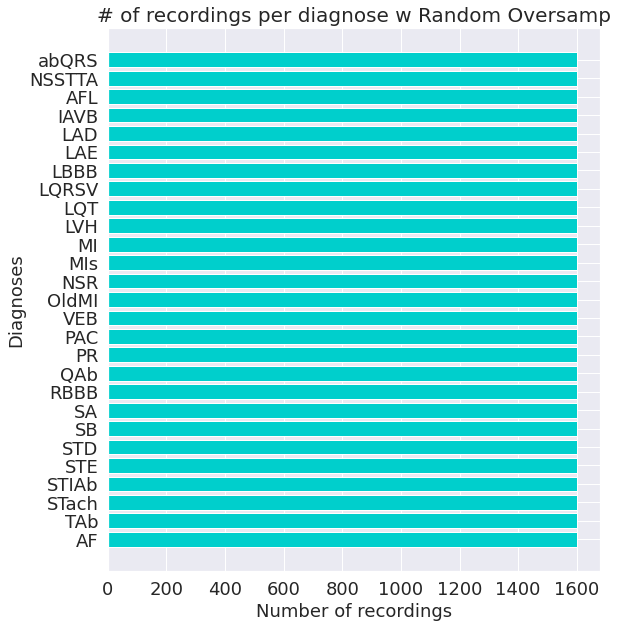
\includegraphics[scale=0.4]{img/label_distro_ros.png}
\caption{Number of recordings for each diagnosis by database for the ROS oversampled data}
\label{fig:label_distro_ros}
\end{figure}

Then, two oversampling methods were proposed to deal with the imbalance issue. The first one is called \textbf{Random Oversampling (ROS)}. In the latter, the minority classes are replicated together with their features. Besides, a down-sampling was applied to have several recordings similar to the filtered dataset. In the end, the ROS dataset had 43,200 recordings. And as depicted in figure \ref{fig:label_distro_ros}, the distribution of the labels is much more similar among the arrhythmia categories.

\begin{figure}[H]
\centering
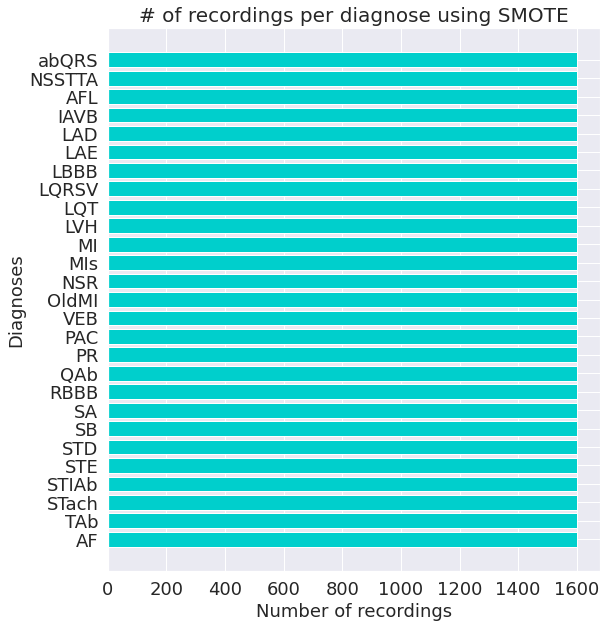
\includegraphics[scale=0.4]{img/label_distro_smote.png}
\caption{Number of recordings for each diagnosis by database for the SMOTE oversampled data}
\label{fig:label_distro_smote}
\end{figure}

The second oversampling technique used was SMOTE (SMT) \ref{3unbclass}. In the end, the SMOTE dataset had also 43,200 recordings. And as shown in figure \ref{fig:label_distro_smote}, the distribution of the labels is also similar among the arrhythmia categories.

\subsection{Fitted models and results}

With the previous pre-processing applied over the data, the following step was to adjust some Machine Learning models to the ECG's arrhythmias. During this step also other scenarios and considerations were employed \cite{datasplit}. A detailed explanation of the outlines is discussed in table \ref{table:scenarios_models}.

\begin{table}[H]
\begin{center}
\begin{tabular}{ ||p{3cm}||p{5cm}||p{4cm}|| }
 \hline
\textbf{Characteristic} & \textbf{Scenarios} & \textbf{Best approach}\\ [0.4ex] 
 \hline\hline
 Data Split & \%Train-\%Validation-\%Test: Option 1: 60\%-20\%-20\% Option 2: 70\%-10\%-10\% Option 3: 80\%-10\%-10\% Option 4: 90\%-5\%-5\% & Option 4: 90\%-5\%-5\%\\
\hline
Features normalization & Option 1: MinMaxScaler \hspace{10 mm} Option 2: StandardScaler \hspace{10 mm} Option 3: RobustScaler & Option 3: RobustScaler \\
\hline
Sampling rate & Option 1: 257Hz \hspace{10 mm} Option 2: 500Hz & Option 1: 257Hz \\
\hline
Features employed & Option 1: Baseline features Option 2: Baseline features + Spectral features & Option 2: Baseline features + Spectral features \\
\hline\hline
\end{tabular}
\end{center}
\caption{Scenarios tried during modelling phase}
\label{table:scenarios_models}
\end{table}

In the previous table are depicted the best approaches that managed to get the best performances (in terms of Accuracy, Recall, Precision, F1-Score and Overall Score). Moreover, in figure \ref{fig:cl_oindex_methods} is shown the detailed behaviour of each one of the algorithms employed.

\begin{figure}[H]
\centering
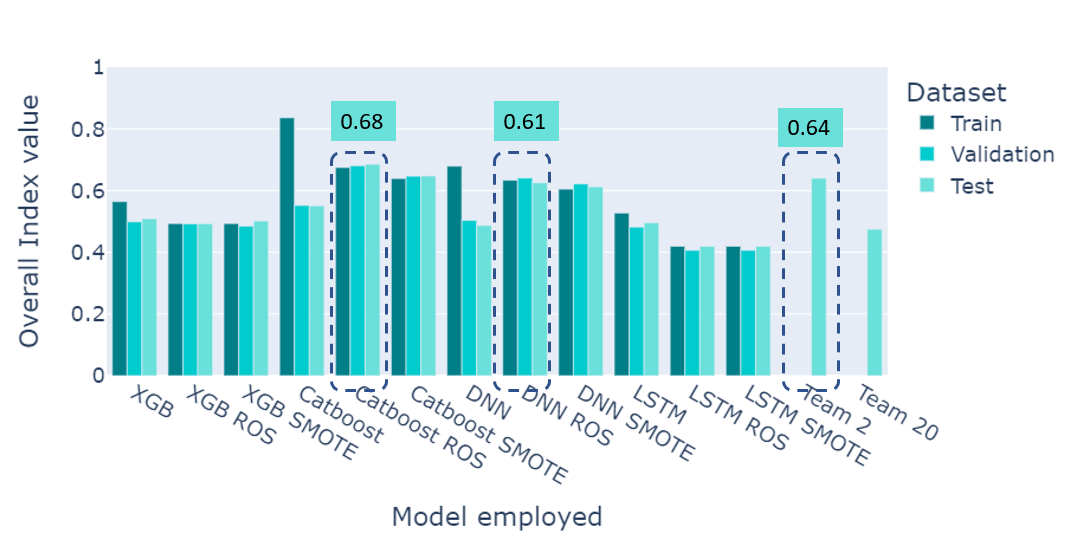
\includegraphics[scale=0.5]{img/cl_oindex_methods.png}
\caption{Overall Index for methods employed in Centralized Learning (CL)}
\label{fig:cl_oindex_methods}
\end{figure}

Within the previous results, it is easy to realize that the champion model is the one that applies Catboost over the ROS data. The latter obtained an overall index close to 0.68. The competition team which ranked 2 is at the second position having an overall index of 0.64. This model has been trained over the above \ref{table:scenarios_models} scenario having trained data as 90\%, 5\% validation data and 5\% for testing and the same pattern has been followed on team 20 analysis. Nevertheless, the Deep Neural Network (DNN) applied over the ROS data has a close behaviour, having a mentioned metric of 0.61. Finally, LSTM and XG-Boost do not perform that well compared to the other models. An additional point to mention is that both Catboost and DNN used over the ROS dataset do not show any sign of overfitting since the metrics for train, validation and test sets are almost the same. As for team 2 and team 20 in the above figure train and validation overall index is not shown because they followed their pattern keeping in mind the competition score during training and validation. 

\begin{figure}[H]
\centering
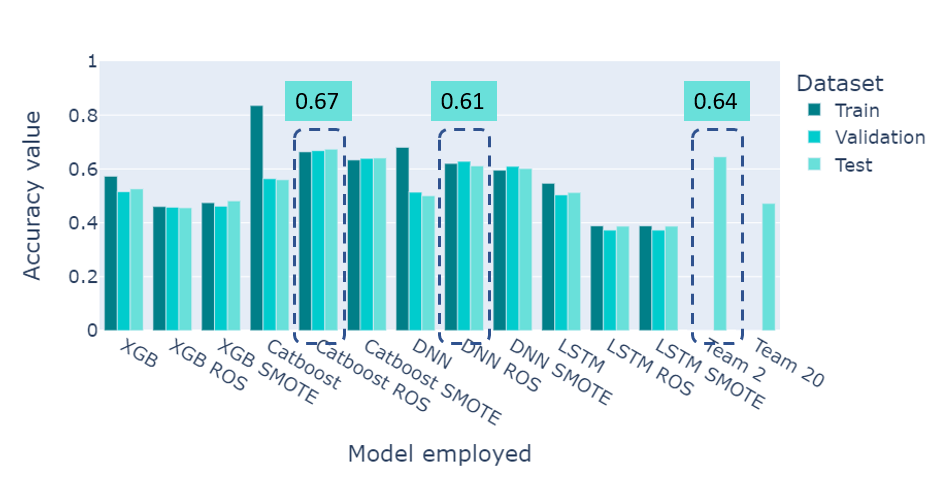
\includegraphics[scale=0.55]{img/cl_accuracy_methods.png}
\caption{Accuracy for methods employed in Centralized Learning (CL)}
\label{fig:cl_accuracy_methods}
\end{figure}

\newpage

\begin{figure}[H]
\centering
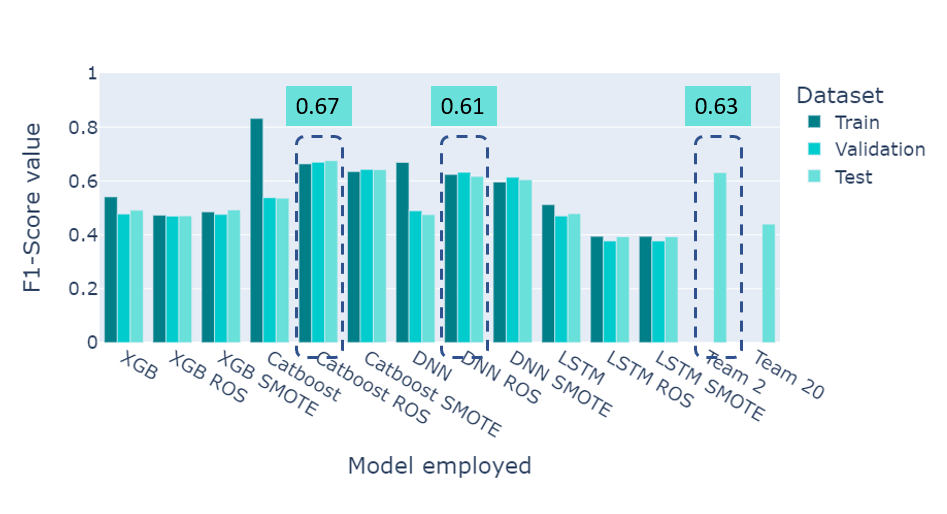
\includegraphics[scale=0.55]{img/cl_f1score_methods.png}
\caption{F1-Score for methods employed in Centralized Learning (CL)}
\label{fig:cl_f1score_methods}
\end{figure}

A similar analysis can be derived from figures \ref{fig:cl_accuracy_methods} and \ref{fig:cl_f1score_methods}, where the Accuracy and F1-Score are shown. In terms of Accuracy, Catboost got 0.67, team 2 got 0.64 and DNN got 0.61 while applied over the ROS dataset. It is important to clarify that using Accuracy is not the best metric in this dataset since the labels are heavily unbalanced. For that reason, it is better to use the F1-Score. which is more robust to the imbalanced datasets. Then, in terms of F1-Score, Catboost obtained a 0.67, the team 2 model got 0.63 and DNN 0.62.

\begin{figure}[H]
\centering
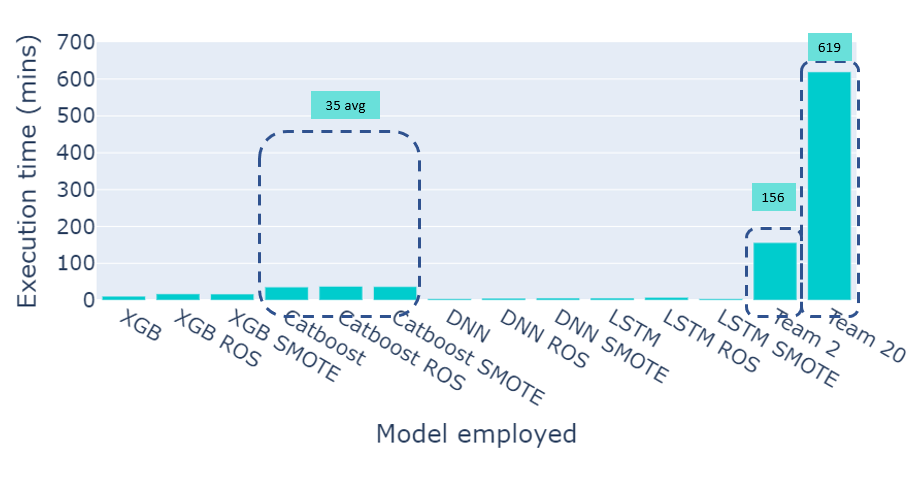
\includegraphics[scale=0.58]{img/time_cl_teams.png}
\caption{Execution times for the methods used in CL}
\label{fig:times_cl}
\end{figure}

Finally, a measurement of the time taken to train for each model was included. As shown in figure \ref{fig:times_cl}, Team 20 model took almost 619 minutes, team 2 took 156 minutes and Catboost took almost 35 minutes to run. On the other hand, DNN and LSTM are algorithms that are employed a few times in training (close to 4 minutes on average). Finally, Catboost is the slowest method, although it generates the best results. In the counter position, DNN is the fastest method, and the performance is NOT quite different from Catboost and the team 2 model. Team 2 and team 20 models took this much time because they are end-to-end models instead of the feature-based model. Although I have done some experiments on team 2 which will be explained below. 


\section{Conversion to Tensorflow Lite } \label{5CTL}

 We can convert potentially any model that is built using TensorFlow core libraries and tools. Once you've built a model with TensorFlow core, you can convert it to a smaller, more efficient ML model format called a TensorFlow Lite. Also, there are other advanced steps related to it if your model is built using TensorFlow core libraries by looking at the steps here  \ref{fig:model_conversion_process} we can convert models that are built using either Pytorch or Matlab. 
 
 
\subsection{Model 1(XGBoost) and Model 2(Catboost) conversion}\label{5CTLM1M2}

As both of \href{https://xgboost.readthedocs.io}{XGBoost} and \href{https://catboost.ai}{Catboost} are not built using Tensorflow even there is no direct conversion available I opted out to use trained models built on top of CatBoost and XGBoost. Just to keep in mind that both of these libraries somehow support directly or indirectly the iOS platform but not the android. After conversion, I am going to use them directly on both iOS/Android to see how they perform in real world scenarios. 

\subsection{Model 3(LSTM)}\label{5CTLM3}

LSTM model is built on top of Tensorflow so it was convertible to TensorFlow lite. If we look at LSTM models of simple LSTM, LSTM ROS, LSTM SMOTE, a better F1-score and overall index are achieved by simple LSTM model with a 0.49 overall index and 0.47 F1-score. LSTM had one problem during the conversion step it had two subgraphs that are not supported by TensorFlow lite models. To overcome this problem \textbf{TFLite LSTM op } was used and in the end, we get the graph that had only one subgraph.


\begin{figure}[H]
\centering
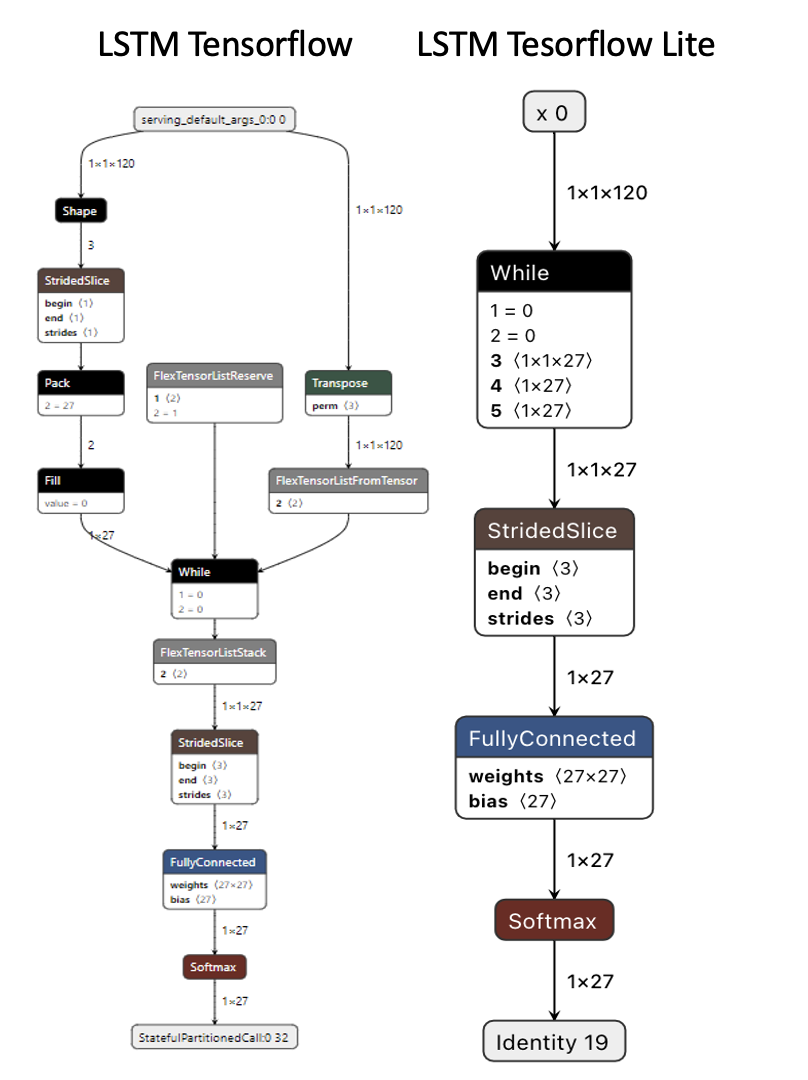
\includegraphics[scale=0.7]{img/lstm_conversion_comparison.png}
\caption{Tensorflow LSTM model's graph to Tensorflow Lite model's graph comparison}
\label{fig:lstm_conversion_comparison}
\end{figure}


As you can see in \ref{fig:lstm_conversion_comparison}, LSTM Tensorflow original model and TensorFlow Lite model after the conversion step has taken place using TFLite LSTM op. 

\subsection{Model 4(DNN)}\label{5CTLM4}

As DNN model was also built using Tensorflow with 4 fully connected layers 3 with 500 neurons output in each and relu as activation function with output. In the fourth layer, it has to output 27 classes of arrhythmias with probabilities so it uses Softmax in the last layer. To look at its graph in the TensorFlow lite model it is not that interesting and the only interesting thing to note is that TensorFlow lite as I have converted only supports one input at a time and Tensorflow one can support batches of inputs as well. As I have to use the TensorFlow Lite version on mobile so most probably it will be given an input to classify one at a time. 


\begin{figure}[H]
\centering
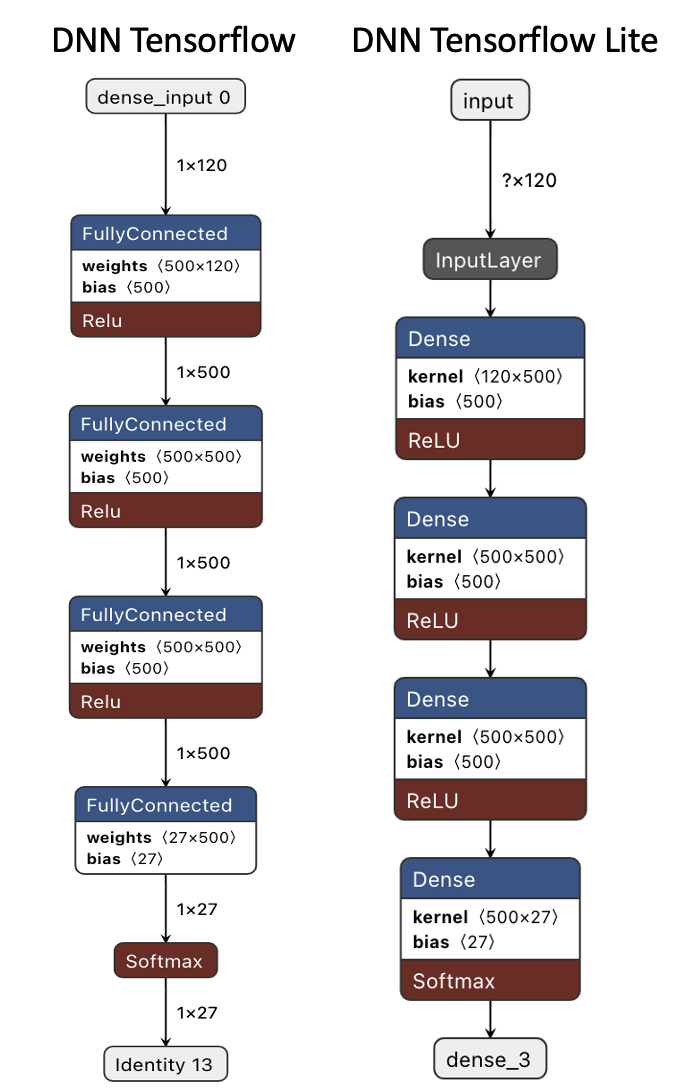
\includegraphics[scale=0.7]{img/dnn_conversion_comparison.png}
\caption{Tensorflow DNN model's graph to Tensorflow Lite model's graph comparison}
\label{dnn_conversion_comparison}
\end{figure}


\subsection{Model 5 - Challenge Team 2}\label{5CTLM5}

As challenge 2 team was using Pytorch instead of Tensorflow as a primary framework library to build the model. I have to convert the model following all the steps mentioned in \ref{fig:model_conversion_process}. So, the first trained model .pt file is converted to ONNX format and gets tested, then it got converted to .pb file and at the end when .pb gets imported to TensorFlow it got directly converted to Tensorflow lite. As challenge team 2 was using an ensemble approach where they were using 5 models which got trained over a shuffled dataset for training and validation. We will look at the first model in .pt format, how it looks and then converted the model in Tensorflow Lite as a comparison. Also, this model length is too big to compare here, I will be using the first few layers as a comparison here. 

\begin{figure}[H]
\centering
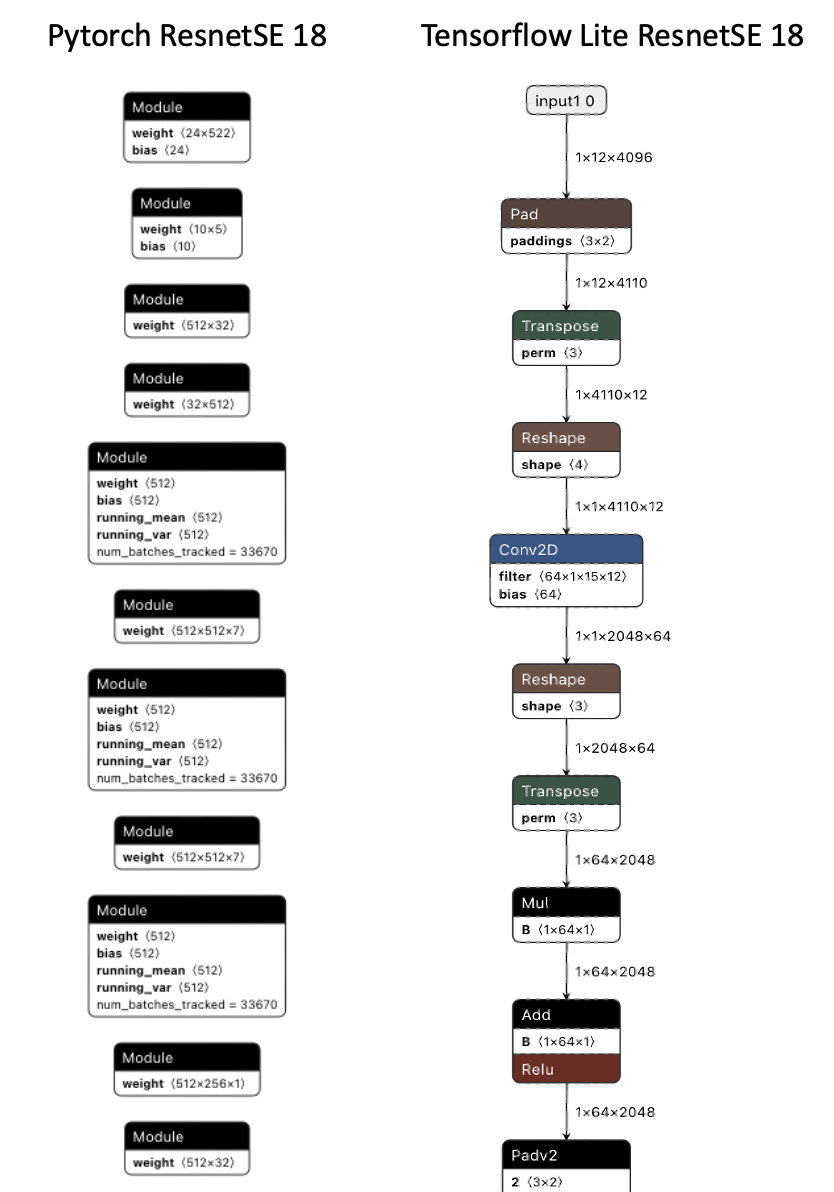
\includegraphics[scale=0.7]{img/resnetse_conversion_comparison.png}
\caption{Pytorch ResnetSE 18 model's graph to Tensorflow Lite model's graph comparison }
\label{resenet18_conversion_comparison}
\end{figure}

As we can see in \ref{resenet18_conversion_comparison} during conversion to TensorFlow Lite there are too many operations that get performed including pad, Transpose, Reshape, Mul, etc. So, we can conclude that in the conversion process to Tensorflow Lite there are additional operations get added to model graphs to support some of the complex operations. 


\subsection{Model 6 - Challenge Team 20}\label{5CTLM6}

As Challenge team 20, worked directly on the Tensorflow framework library it was easy to convert the model to Tensorflow Lite directly. Let's look at the original model and converted model comparison side by side. It is also important to mention that as they were training 10 different models using a shuffled dataset and I choose the one for comparison which was performing better in Accuracy, F1-Score and the overall index. It is important to note that the difference between these models was really small in terms of metrics as mentioned before. Model graph length is too big to paste it here so I will be comparing the first few layers of it as in the case of Model 5. \ref{5CTLM5} 


\begin{figure}[H]
\centering
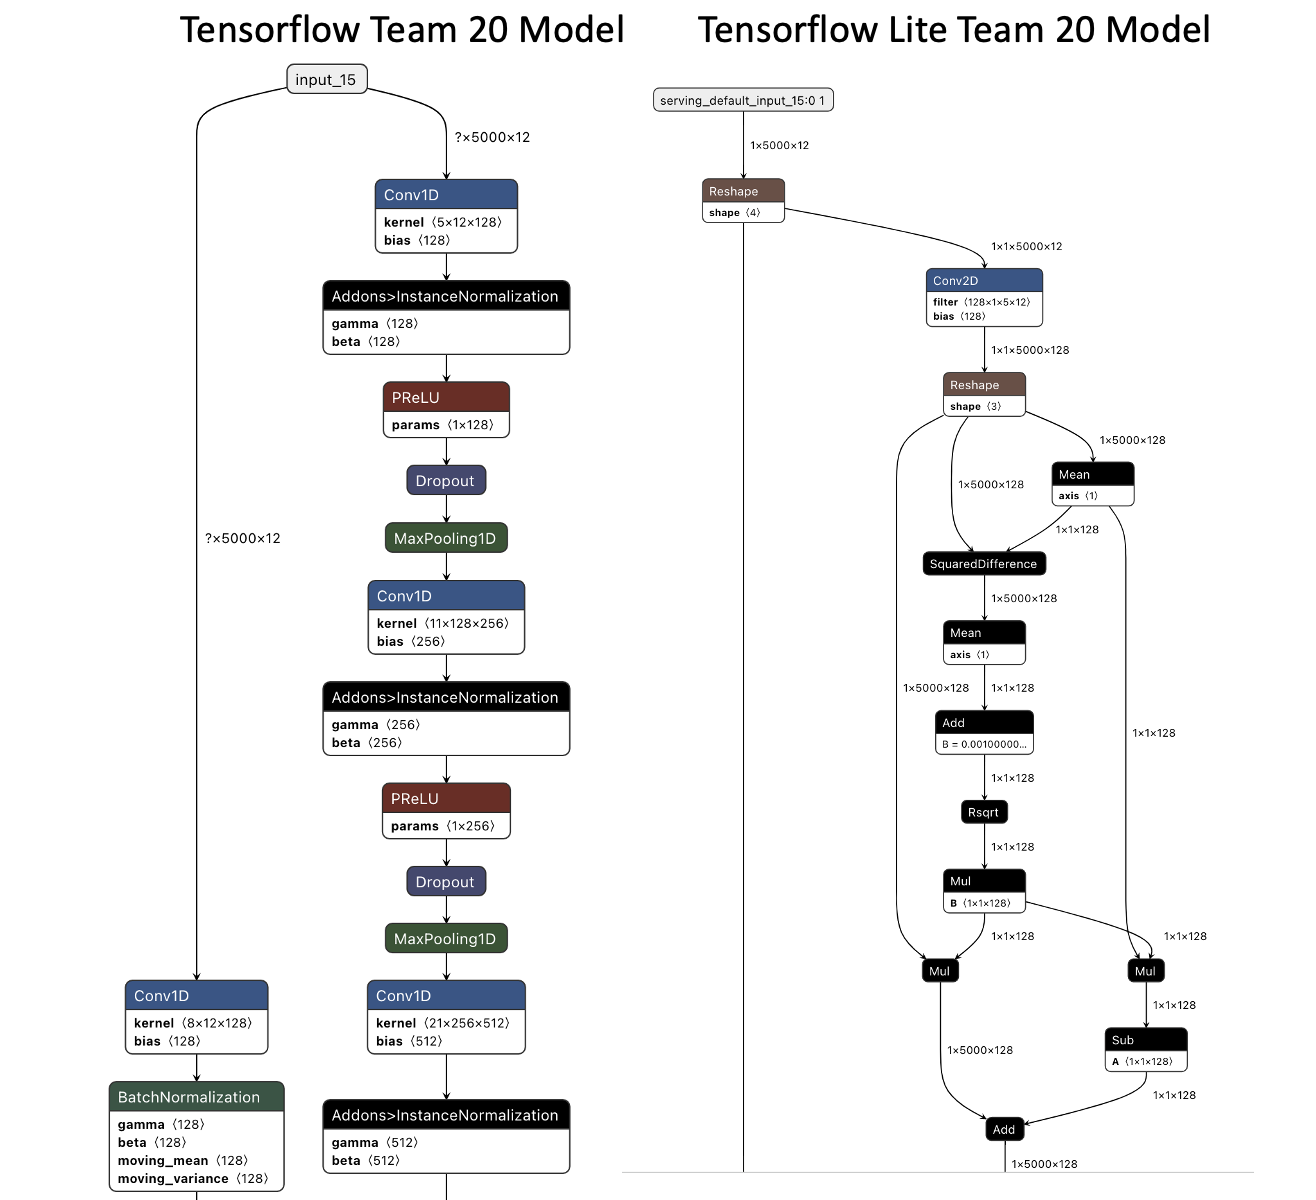
\includegraphics[scale=0.65]{img/team20_conversion_comparison.png}
\caption{Tensorflow Team 20 model's graph to Tensorflow Lite model's graph comparison}
\label{team20_conversion_comparison}
\end{figure}

Looking at the above figure \ref{team20_conversion_comparison}, we can clearly see that in the TensorFlow Lite graph there are multiple other operations that we haven't seen before like Sub, SquaredDifference, Mean, Rsqrt etc. It is evident all the complex operations get converted to simpler operations in the TensorFlow Lite format of the model.  



\subsection{Metrics of models}

As written previously, Catboost and XGBoost \ref{5CTLM1M2} are not convertible directly to TensorFlow Lite. Besides, those other models were convertible and it was only worth looking at the models that performed well in terms of accuracy, f1-score and overall index because they will be later used for detecting arrhythmias in mobile applications. So, DNN ROS with an overall index of 0.62, LSTM with an overall index of 0.49, Team 2 model with an overall index of 0.64 and Team 20 model(CNN+Rule Based) with an overall index of 0.47 was chosen for the below analysis. 


\begin{figure}[H]
\subfloat[DNN ROS]{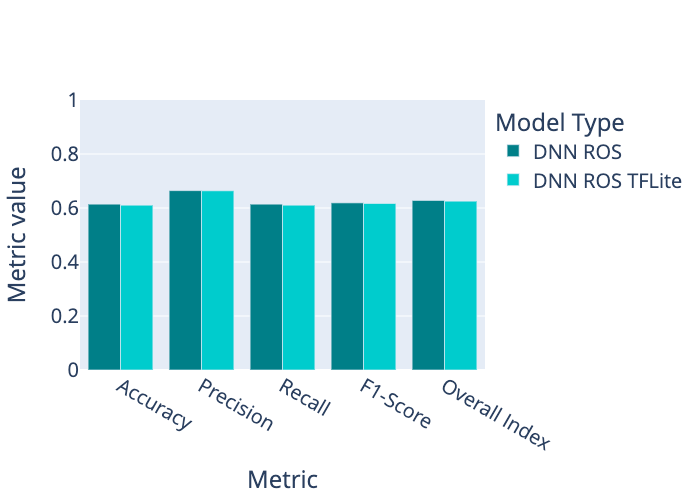
\includegraphics[width = 2.8in]{img/dnnros_metrics.png}} 
\subfloat[LSTM]{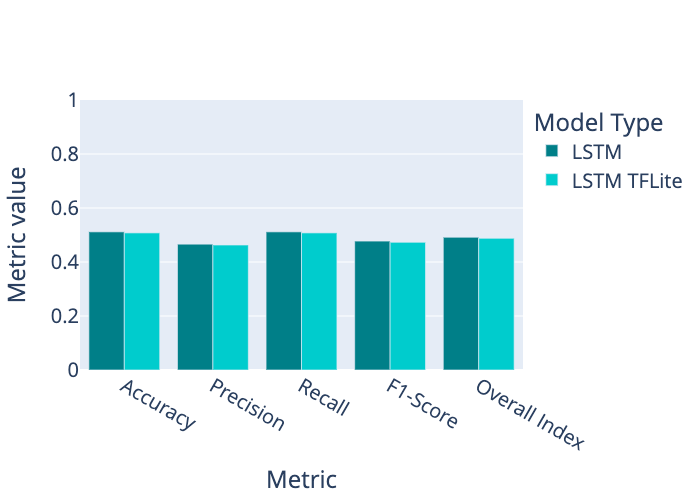
\includegraphics[width = 2.6in]{img/lstm_metrics.png}}\\
\subfloat[Team 2]{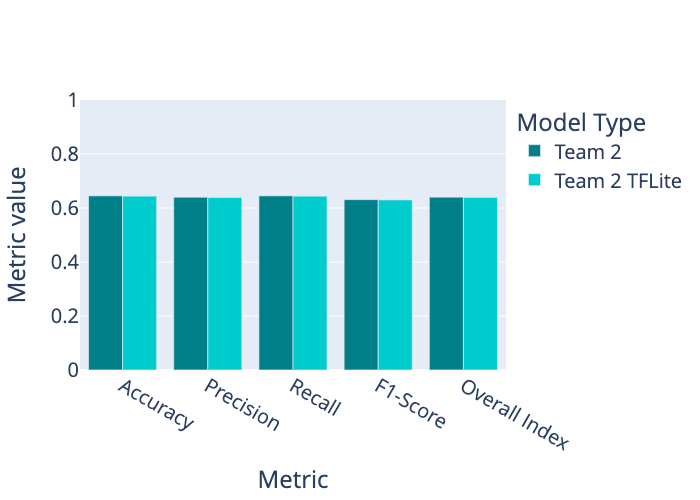
\includegraphics[width = 2.7in]{img/team2_metrics.png}}
\subfloat[Team 20]{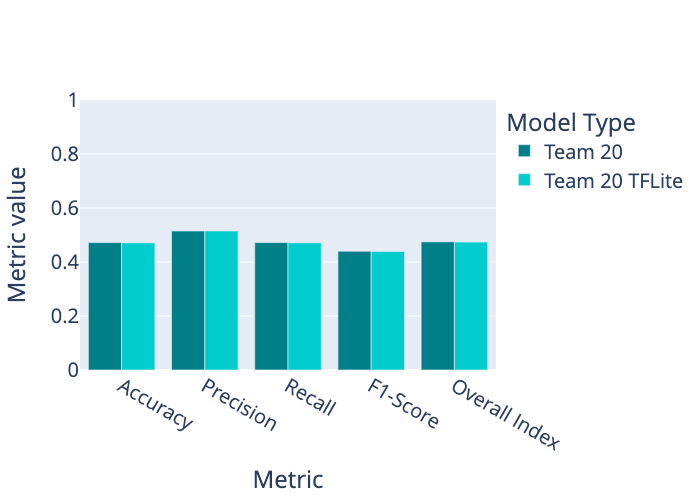
\includegraphics[width = 2.8in]{img/team20_metrics.png}} 
\caption{Metrics of models comparing side by side with original model and TF Lite version of the model}
\label{metricsafterconversion}
\end{figure}

If we look at the above figures we can clearly see a little drop in every metric after the model is converted to TensorFlow Lite. As, I didn't want the models to be quantised more so that their accuracy, and F1-Score decrease so I opted for TensorFlow Lite default conversion operations. 


Now if we move toward looking at how much time it takes to get output from the model either before converting or after converting. There is huge difference when a model is converted and we wanted to get the output from the model. It takes slightly and in the case of the hefty model, it takes a lot more time. In real world scenario as we will not be using batching, or multiple inputs to get the output from the model because all above-converted models only accept one input at a time. 

\begin{figure}[H]
\centering
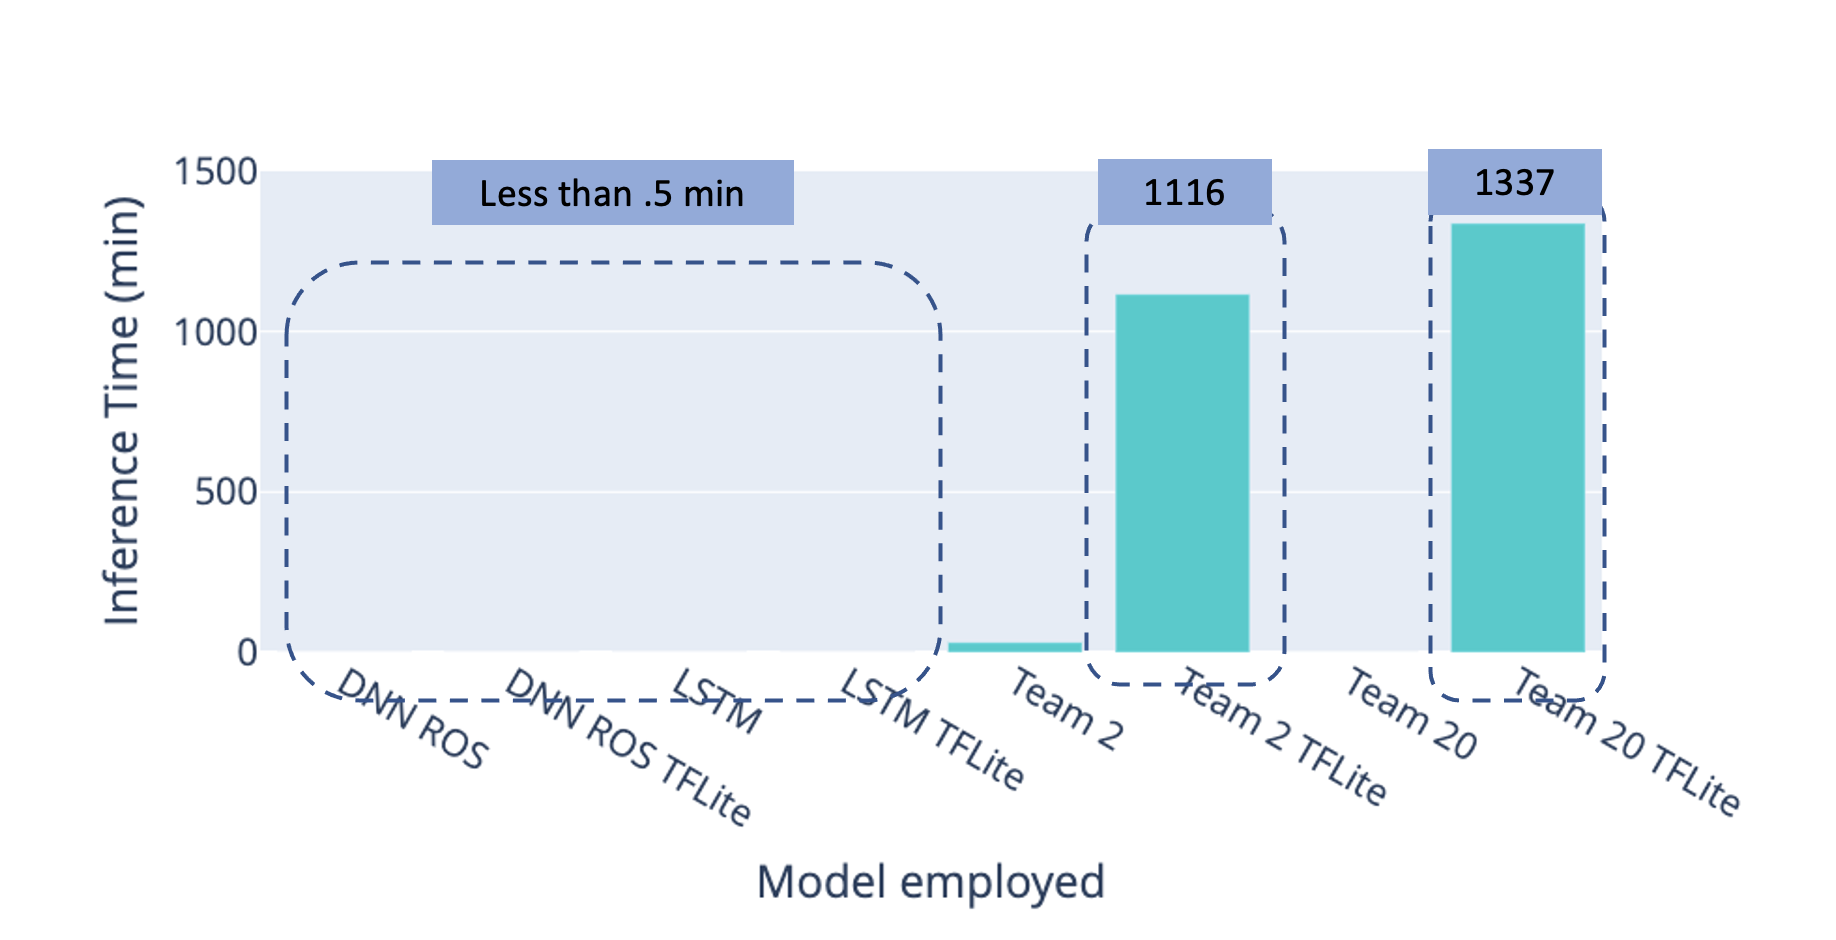
\includegraphics[scale=0.45]{img/inference_time_of_converted_models.png}
\caption{Inference Time in minutes of original and converted models}
\label{inference_time_of_converted_models}
\end{figure}

If we look at the above \ref{inference_time_of_converted_models} figure we can clearly see that LSTM and DNN ROS models are way faster than Team 2 and Team 2. LSTM and DNN ROS models even after conversion is taking less than 0.30 sec to execute. To put it more precisely original DNN on a test dataset with 2095 features takes 19 seconds to get outputs and .13 seconds for inference in the case of a converted model which is even less than the original model. If we look at LSTM it does the same 13 seconds for the original model and .067 seconds on the converted model. This means that somehow both DNN and LSTM have to perform fewer operations and get lighter and more efficient after conversion. While on the other hand Team 2 and Team 20 models take significantly too much time to output the results. More precisely, in the case of the Team 2 model, it takes 1826 seconds to output 2095 results and 66960 seconds in the case of the converted model which raises concerns because it is significantly slower than the original model. As in the case of team 20 inference on the original model was significantly smaller at 9.4 seconds and inference on the converted model was huge slower at 80232 seconds. It may be due to CPU or GPU inference, I didn't get a chance to look at it. 

\begin{table}
\centering
\begin{tabular}{ |p{5cm}||p{3cm}|p{3cm}|}
 \hline
 \multicolumn{3}{|c|}{Size of Models} \\
 \hline
 Model's Name& Original Size&Converted size\\
 \hline
 DNN ROS   & 2.2MB   &   569KB\\
 LSTM&  \textbf{82KB}   & \textbf{29KB} \\
 TEAM\#2 &33.8MB & 9.6MB\\
 TEAM\#20  & 138.8MB & 11.6MB\\
 \hline
\end{tabular}
 \caption{\label{tab:models_size_after_conversion}Comparison of model size from original to converted models}
 \end{table}
 
 As you can see from \ref{tab:models_size_after_conversion}, the smallest model is LSTM and it even gets smaller when converted to TensorFlow lite. Team \#20 model is really huge and it gets converted to 11.6MB. Maybe because of that it takes time during inference. 
 
\subsection{Models Deployment}\label{modelsdeployment}

As part of the model testing on mobile devices after conversion. LSTM, DNN ROS and Team \#2 model have been deployed on the mobile devices while building a small demo application using flutter. \href{https://flutter.dev/}{Flutter} is an open-source UI software development kit created by Google. As flutter supports Tensorflow Lite models only Catboost, XGBoost are not deployed, as well as the Team \#20 model because the accuracy, F1-Score of the team \#20 model is very less. 

In the demo application, two main packages has been used \href{https://pub.dev/packages/tflite\_flutter}{tflite\_flutter} and \href{https://pub.dev/packages/csv}{csv}. \textit{csv} package has been used to read csv files and \textit{tflite\_flutter} is used to inference converted models. 

\textbf{DNN ROS and LSTM}

For DNN ROS and LSTM, I saved the features of the test dataset 5\% after normalizing and standardizing as explained above \ref{5fsn} in the csv file. This csv file is used directly for inputs to the models. Then as both models are trained to classify single arrhythmia. The output of the model is based on classifying 27 arrhythmias so whichever arrhythmia type is at the highest probability is shown as predicted and then two more types according to the highest probabilities are shown in \ref{dnn_deloyment} 

\newpage 


\begin{figure}[H]
\centering
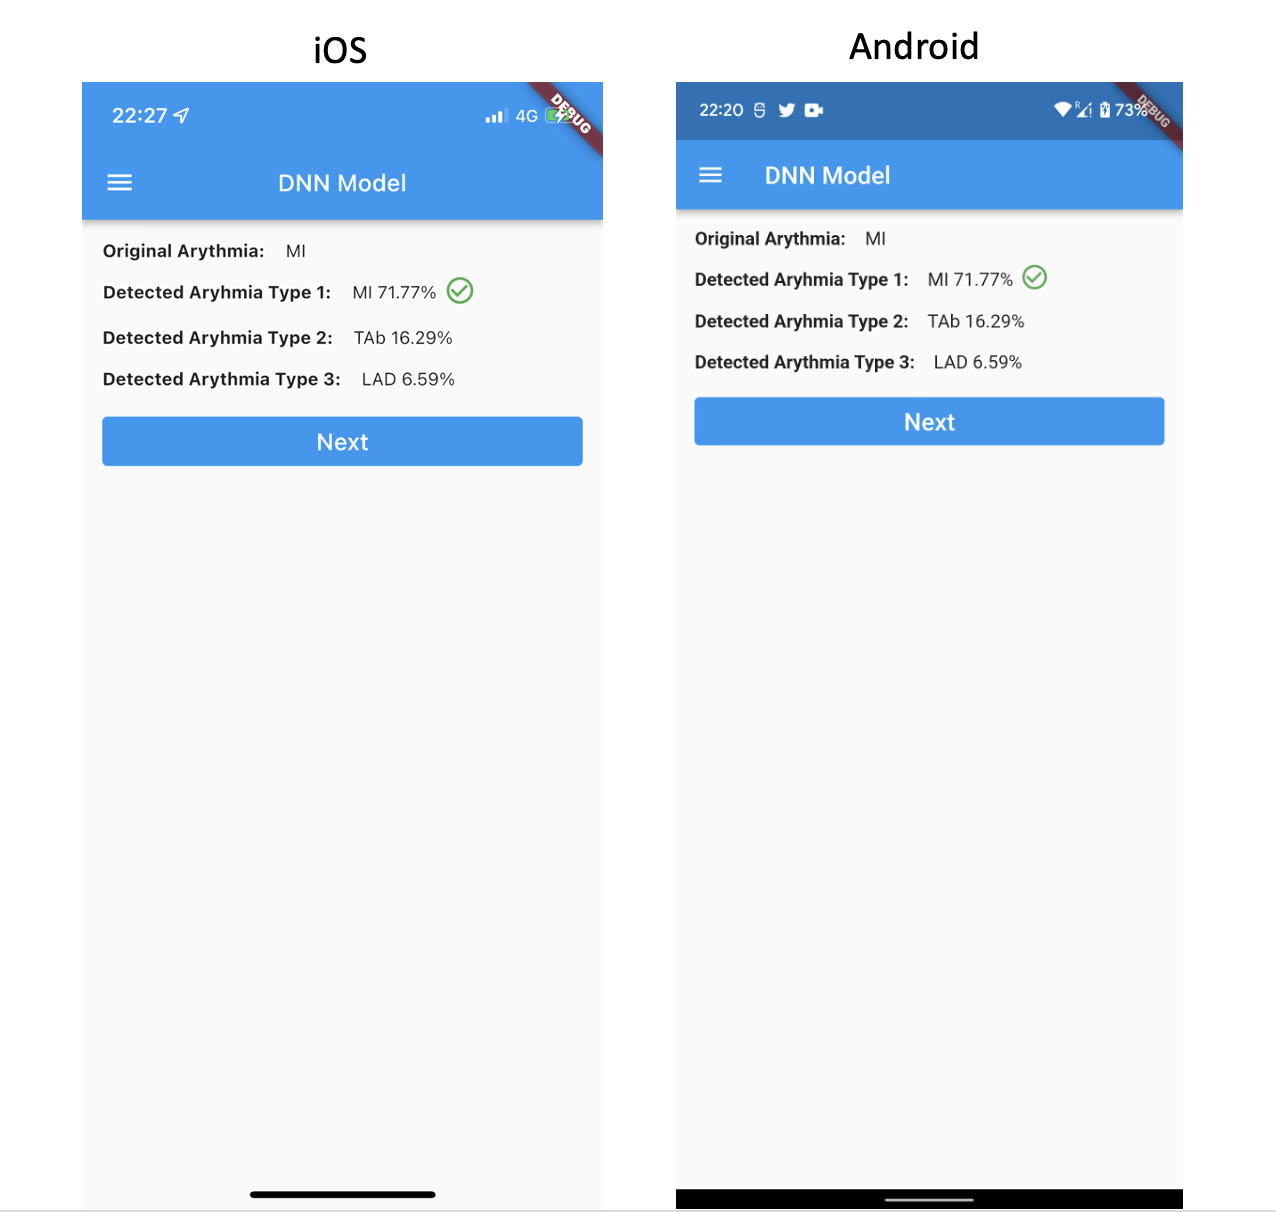
\includegraphics[scale=0.4]{img/dnn_deloyment.png}
\caption{iOS and Android DNN model classification example}
\label{dnn_deloyment}
\end{figure}

\begin{figure}[H]
\centering
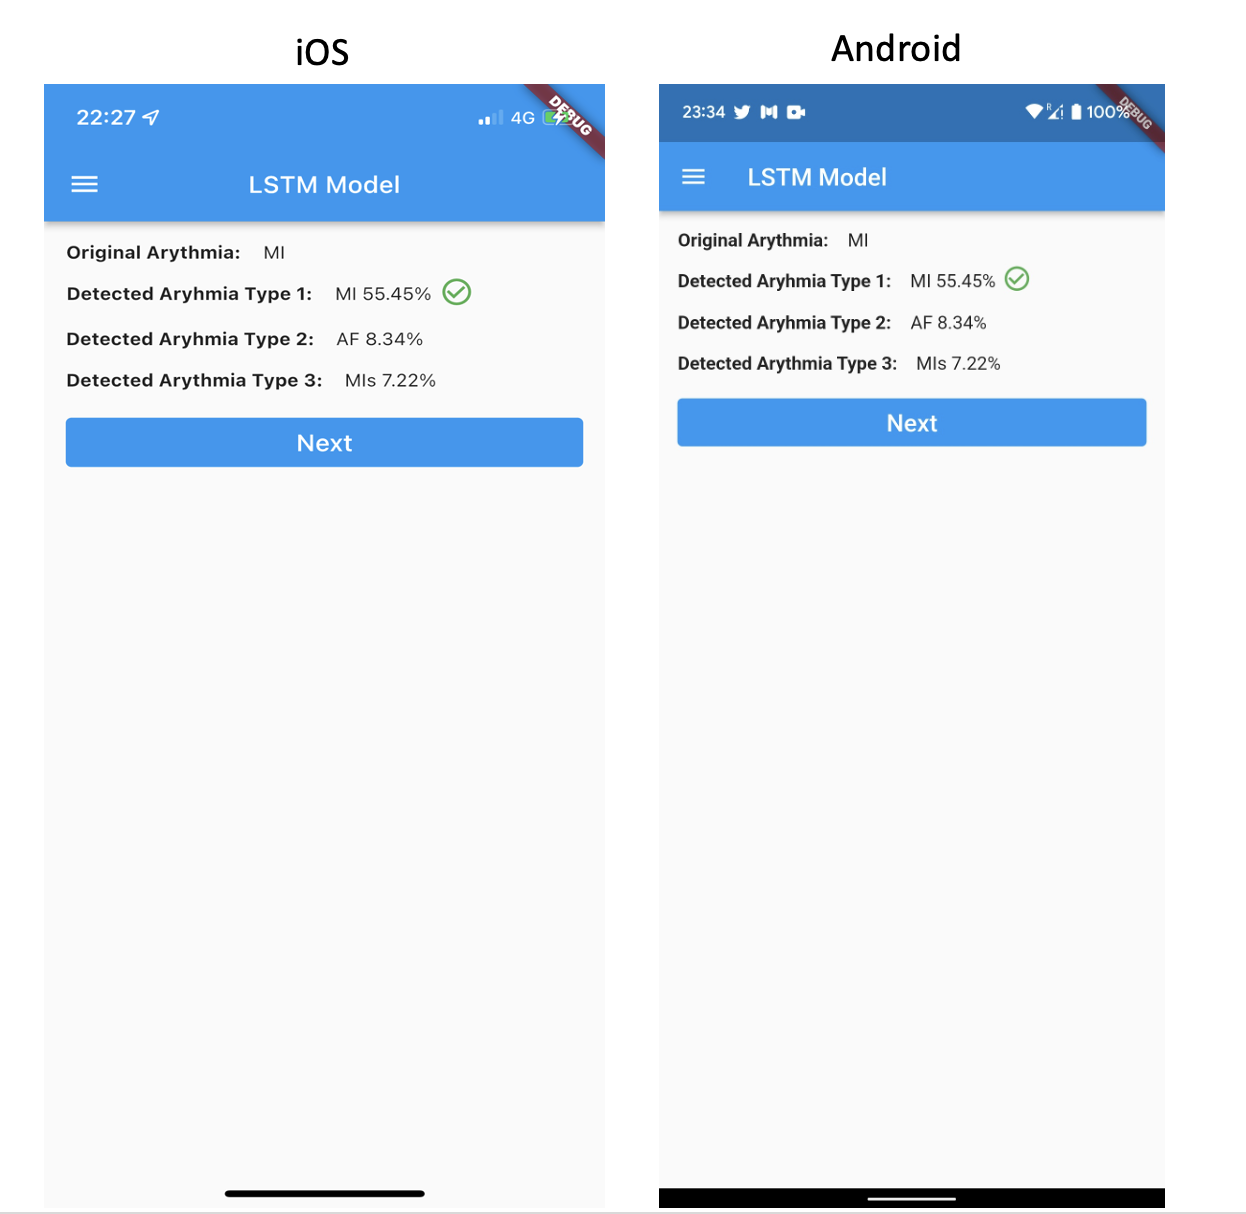
\includegraphics[scale=0.4]{img/lstm_deployment.png}
\caption{iOS and Android LSTM model classification example}
\label{dnn_deloyment}
\end{figure}

\textbf{Competence Team \# 2}

For competence team \# 2, as they were using end to end model to classify 12-lead ECG, so for each input after pre-processing was saved as one csv file instead .mat file in the original dataset and age, sex and dx is saved separately as well in another csv file to provide it to the model. As competence team \# 2 was using ensemble model, combining 5 of them to output the results for final classification there have been post-processing done on the mobile application as it was in original source code provided by \ref{fig:team_two_network_2}. If we look closely their model is doing multi-class classification instead of predicting one arrhythmia at a time because a patient can have more than one arrhythmia. Also, during prediction probabilities are divided into a combination of the percentage for how many arrhythmias it predicts. For example, if the model is predicting two different arrhythmias based on 12-lead ECG it will make the whole percentage as 200\% instead of 100\%. 

\begin{figure}[H]
\centering
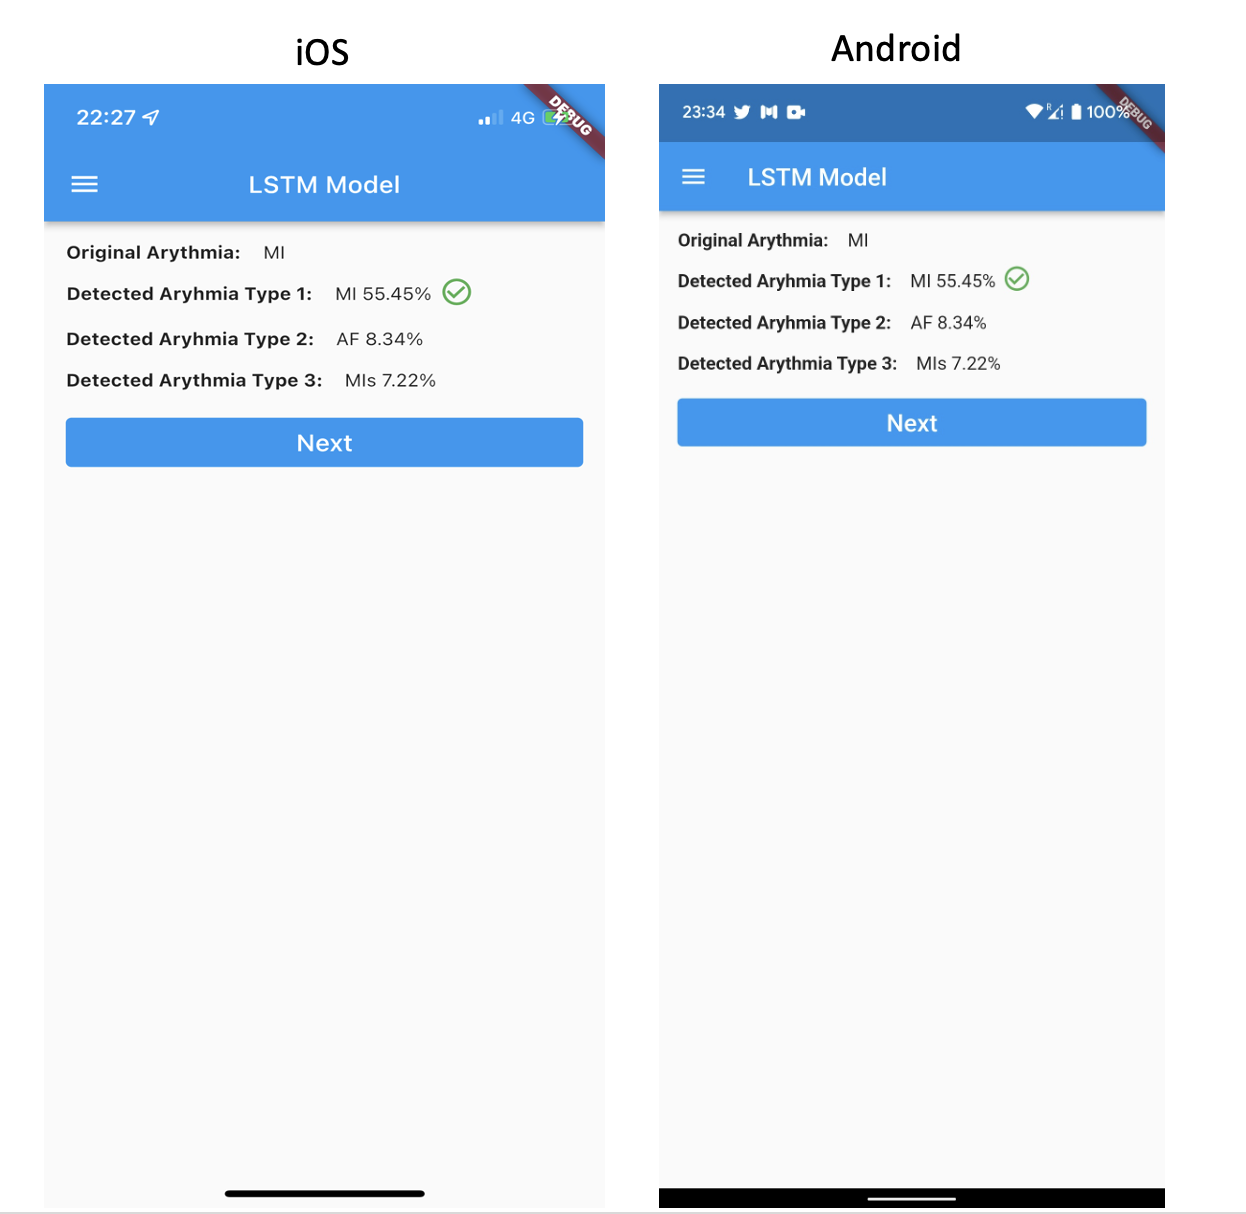
\includegraphics[scale=0.4]{img/lstm_deployment.png}
\caption{iOS and Android Team \# 2 model classification example}
\label{dnn_deloyment}
\end{figure}




\section{Federated Learning} \label{5FL}

Leveraged on the Centralized Learning method mentioned, it is time to immerse in the Federated Learning (FL) approach executed for this ECG dataset. With the CL it was possible to get an overall performance with the best technique and scenarios to be applied. To deal with the FL proposed IID approach has been chosen for analysis. 

\subsection{IID approach}

This approach was based on the idea of using the whole dataset containing 41,894 registers and dividing it into 4 different datasets (local nodes). As a parenthesis, the decision of the number of local nodes was based on selecting at least 30 diagnoses for the rarest arrhythmia. Due to the stratified random splitting, the mentioned data in each local node (or client) will be Independent and Identically Distributed (IID) \ref{proposed_approaches}. This scenario is not completely realistic since usually the ECGs shared in multiple devices are Non-IID. Nevertheless, it is worth trying and seeing how the FL approach will perform over the data.

\begin{figure}[H]
\centering
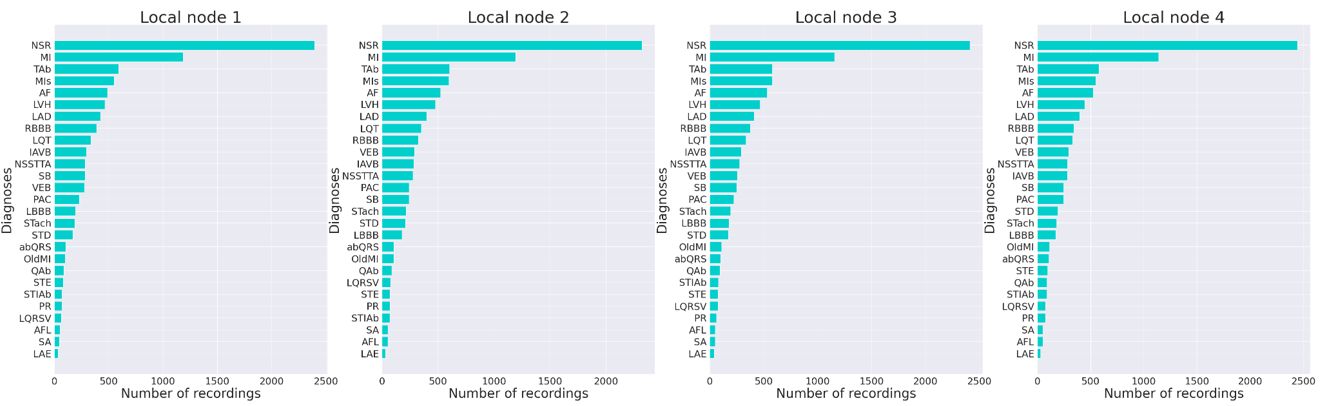
\includegraphics[scale=0.4]{img/fl_label_distro_filtered.png}
\caption{Label distribution for the filtered dataset by each local node}
\label{fig:fl_label_distro_filtered}
\end{figure}

As depicted in figure \ref{fig:fl_label_distro_filtered}, the distribution among the 4 local nodes seems IID. The latter means that the diagnoses along the devices will be the same. Besides, each local node contains 9,426 recordings. The same occurs for the ROS and SMOTE datasets when dividing them into 4 clients, as is shown in figures \ref{fig:fl_label_distro_filtered_ROS_SMT}. Of course, in this case, all the diagnoses have almost the same participation across the nodes, making them IID and balanced.

\begin{figure}[H]
\centering
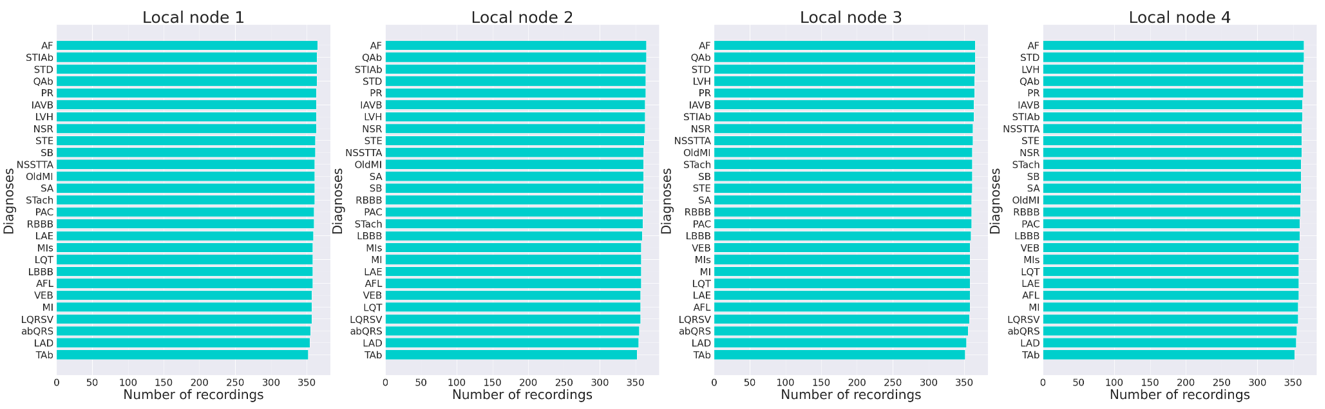
\includegraphics[scale=0.4]{img/fl_label_distro_filtered_ROS_SMT.png}
\caption{Label distribution for the ROS and SMOTE datasets by each local node}
\label{fig:fl_label_distro_filtered_ROS_SMT}
\end{figure}

Once the four datasets were settled, the modelling part can be performed. As a reminder, in the FL technique, each local node will train a model and later it will send the weights to a global node where the weights are averaged and updated back to each client. Then, the DNN and LSTM methodologies were used to classify the ECG's arrhythmias. It is relevant to highlight that Catboost and XG-Boost were not employed in this step. The former was discarded for its low performance and the latter due to its huge training time. Moreover, in the consulted bibliography, it is not common to use those ML techniques within the FL.

\begin{figure}[H]
\centering
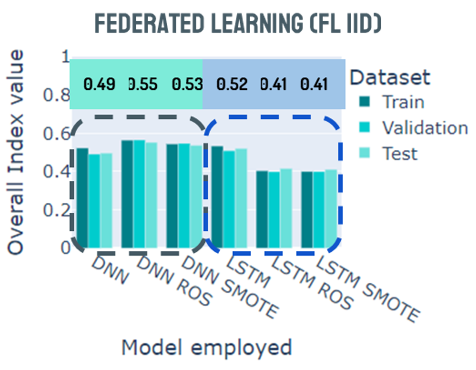
\includegraphics[scale=0.59]{img/fl_iid_methods.png}
\caption{Overall Index for methods employed in Federated Learning (FL)}
\label{fig:fl_iid_methods}
\end{figure}

As depicted in figure \ref{fig:fl_iid_methods}, the best results were obtained using the DNN with the ROS datasets. The latter got an overall index of 0.55 in the test set. On the other hand, the best performance for LSTM was obtained with the original data, although it is worst than the DNN ROS model. The latter means that applying oversampling techniques doesn't improve the result of the models in the LSTM approach. But, when using ROS, the performance of the FL model is the most useful compared to all the techniques.

\begin{figure}[H]
\centering
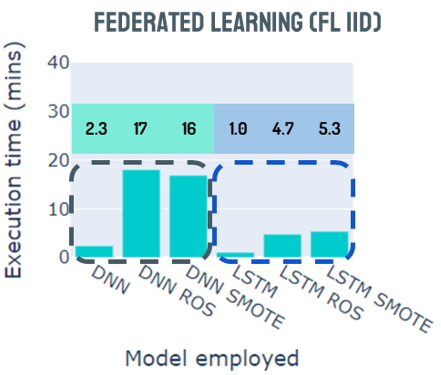
\includegraphics[scale=0.6]{img/times_fl_iid.png}
\caption{Execution times for the methods used in FL IID approach}
\label{fig:times_fl_iid}
\end{figure}

Analyzing figure \ref{fig:times_fl_iid} it is possible to get that the oversampling techniques cause the running time to increase \cite{fl28}. In detail, the slowest approach ended up being the DNN ROS with 17 minutes. Comparing the results to the CL approach, the DNN method with FL runs faster with similar results. On the other hand, DNN ROS and SMOTE ran slower and with a slower performance than the CL. Finally, LSTM, in general, has a lower performance than DNN but runs faster.

With FL it is possible to control the performance that the models have in each local node. The latter is relevant to understand if there is some node that is under-performing, compared to the others.

\begin{figure}[H]
\centering
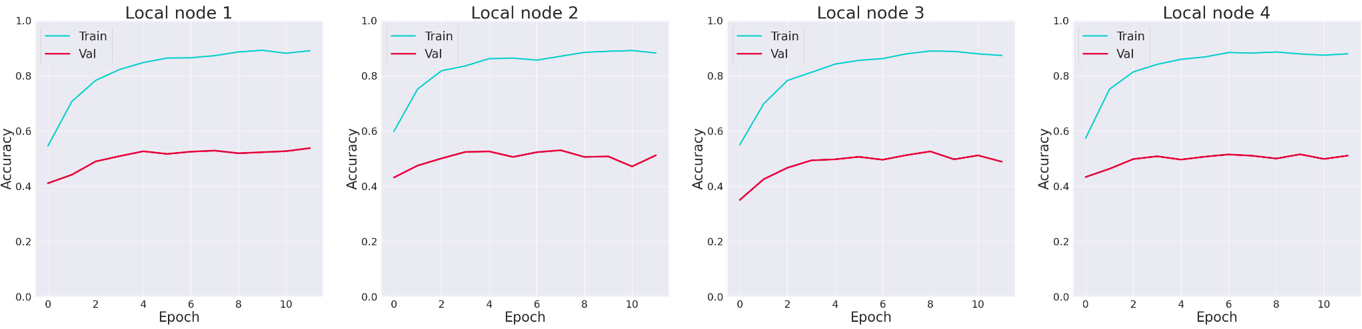
\includegraphics[scale=0.38]{img/iid_local_nodes_acc.png}
\caption{Train and Validation accuracy among local nodes for DNN ROS}
\label{fig:iid_local_nodes_acc}
\end{figure}

In figure \ref{fig:iid_local_nodes_acc} is depicted the behaviour of each local node concerning the accuracy for both the training and validation datasets. In general, the models among the clients have similar behaviour. All of them get stabilized around the 5th epoch. It is important to clarify that the accuracy for train and validation seems considerably far from each other. The latter would mean that the models are over-fitting. Nevertheless, the train sample is an over-sampled data while the validation is a part of the original data, then, it is expected to such behaviour.

In an FL environment, there is a concept called \textbf{communication round} (comm round). The latter begins when a model is trained inside each one of the local nodes. Later the weights of the models are passed to the global node to be aggregated there. And finally, the communication round finishes when each local model is updated with the new weights. Then, it is expected that in each comm round the performance of the model increases. Moreover, it should get stable after some trials.

\begin{figure}[H]
\centering
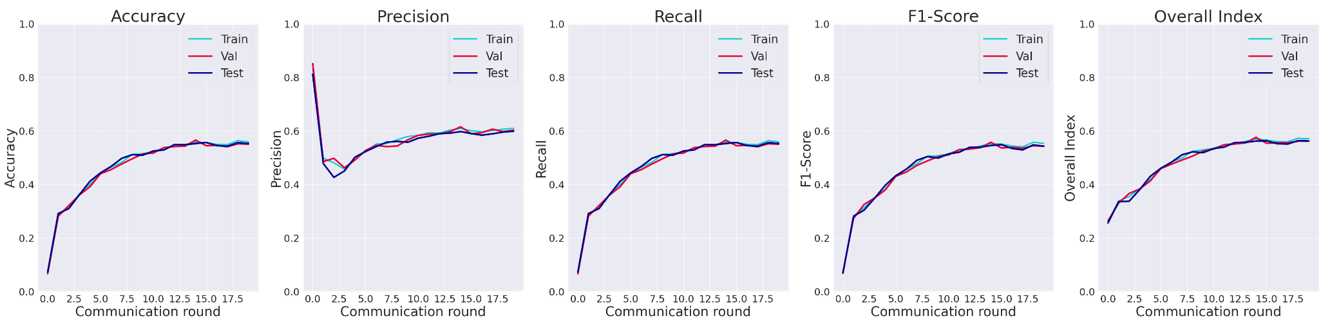
\includegraphics[scale=0.4]{img/comm_round_metrics_DNNROS.png}
\caption{Metrics along communication rounds for DNN ROS (the best model)}
\label{fig:comm_round_metrics_DNNROS}
\end{figure}

Figure \ref{fig:comm_round_metrics_DNNROS} establishes the behaviour of each metric along the communication rounds. As expected, the performance gets stable after the 15th comm round approximately. It is relevant to notice that in the first comm round the Precision starts high and the Recall low. But after some updates both measures get steady. Moreover, the curves for train, validation and test are close. The latter means that there are no signals of overfitting.


\begin{table*}[ht]
\begin{center}
% \begin{tabular}{ ||p{1cm}||p{1cm}||p{1cm}||p{1cm}||p{1cm}||p{1cm}||}
% \resizebox{\width}{!}{
\begin{adjustbox}{width=\textwidth}
\begin{tabular}{|l|*{5}{c}|*{5}{c}|}

\cline{1-11} & \multicolumn{5}{c|}{CL} & \multicolumn{5}{c|}{FL IID}       \\  \cline{2-11}
 Method & \multicolumn{1}{c|}{Accuracy} & \multicolumn{1}{c|}{Precision}& \multicolumn{1}{c|}{Recall}& \multicolumn{1}{c|}{F1-Score} & \multicolumn{1}{c|}{Time} & \multicolumn{1}{c|}{Accuracy} & \multicolumn{1}{c|}{Precision}& \multicolumn{1}{c|}{Recall}& \multicolumn{1}{c|}{F1-Score} & \multicolumn{1}{c|}{Time} \\ 
 \hline \hline
\multicolumn{1}{|l|}{Competence Team \#2 \cite{second_team}} & 0.64 & 0.64 & 0.64& 0.63 & 155 & - & - & - & - & - \\

\multicolumn{1}{|l|}{Competence Team \#20 \cite{team_20}} & 0.47 & 0.51 & 0.47 & 0.44 & 618 & - & - & - & - & - \\
\multicolumn{1}{|l|}{Inspirational DNN \ref{3model4}} & 0.50 & 0.46 & 0.50 & 0.47 & \textbf{1.4} & - & - & - & - & -  \\
\multicolumn{1}{|l|}{Inspirational LSTM \ref{3model3}} & 0.50 & 0.45 & 0.50 & 0.46 & 2.1 & - & - & - & - & -  \\
\hline\hline
\multicolumn{1}{|l|}{XG-BOOST} & 0.52 & 0.49 & 0.52 & 0.49 & 9.4 & - & - & - & - & -  \\
\multicolumn{1}{|l|}{XG-BOOST ROS} & 0.45 & 0.58 & 0.45 & 0.47 & 15.7 & - & - & - & - & - \\ 
\multicolumn{1}{|l|}{XG-BOOST SMOTE} & 0.48 & 0.55 & 0.48 & 0.49 & 15.4 & - & - & - & - & -  \\
\multicolumn{1}{|l|}{CATBOOST} & 0.55 & 0.54 & 0.55 & 0.53 & 34.5 & - & - & - & - & - \\
\multicolumn{1}{|l|}{CATBOOST ROS} & \textbf{0.67} & \textbf{0.72} &\textbf{ 0.67 }& \textbf{0.67} & 36.4 & - & - & - & - & -  \\
\multicolumn{1}{|l|}{CATBOOST SMOTE} & 0.64 & 0.66 & 0.64 & 0.64 & 35.5 & - & - & - & - & -  \\
\hline\hline
\multicolumn{1}{|l|}{DNN} & 0.50 & 0.47 & 0.50 & 0.47 & 2.8 & 0.46 & 0.53 & 0.45 & 0.49 & 2.3  \\
\multicolumn{1}{|l|}{DNN ROS} & 0.61 & 0.66 & 0.61 & 0.61 & 3.8 & \textbf{0.55} & \textbf{0.59} & \textbf{0.54} & \textbf{0.55} & 16.3  \\
\multicolumn{1}{|l|}{DNN SMOTE} & 0.60 & 0.64 & 0.60 & 0.60 & 4.3 & 0.52 & 0.58 & 0.52 & 0.51 & 16.8  \\
\hline\hline
\multicolumn{1}{|l|}{LSTM} & 0.51 & 0.47 & 0.51 & 0.39 & 4.3 & 0.48 & 0.58 & 0.48 & 0.52 & \textbf{1.0}  \\ 
\multicolumn{1}{|l|}{LSTM ROS} & 0.38 & 0.51 & 0.38 & 0.39 & 4.9 & 0.39 & 0.48 & 0.38 & 0.38 & 4.7  \\
\multicolumn{1}{|l|}{LSTM SMOTE} & 0.39 & 0.49 & 0.39 & 0.39 & 2.7 & 0.39 & 0.47 & 0.39 & 0.38 & 5.3  \\
\hline
\end{tabular}
% }
\end{adjustbox}
\end{center}
\caption{Metrics for Centralized (CL) and IID Federated Learning (FL -IID) in the test data set. Also included execution time for training in minutes.}
\label{table:metrics_CL_FLIID}
\end{table*}

The table \ref{table:metrics_CL_FLIID} includes a summary of all the techniques implemented with the data in the IID and Centralized (CL) approaches. It is remarkable to mention that Catboost ROS outperform Competence Team \# 2 model. DNN ROS is a model that has good enough accuracy and f1-score which can be easily deployed to any small memory device after conversion.  